\documentclass[sigconf]{acmart}

\usepackage{booktabs} % For formal tables
\usepackage{listings}

% Copyright
%\setcopyright{none}
%\setcopyright{acmcopyright}
%\setcopyright{acmlicensed}
\setcopyright{rightsretained}
%\setcopyright{usgov}
%\setcopyright{usgovmixed}
%\setcopyright{cagov}
%\setcopyright{cagovmixed}


% DOI
\acmDOI{10.475/123_4}

% ISBN
\acmISBN{123-4567-24-567/08/06}

%Conference
\acmConference[WWW 2020]{The web conference}{April 2020}{Taipei, Taiwan}
\acmYear{2020}
\copyrightyear{2016}


\acmArticle{4}
\acmPrice{15.00}

% These commands are optional
%\acmBooktitle{Transactions of the ACM Woodstock conference}
\editor{Jennifer B. Sartor}
\editor{Theo D'Hondt}
\editor{Wolfgang De Meuter}


\begin{document}
\title{CodeGraph: A knowledge graph for Python code mined from the web}
\titlenote{Produces the permission block, and
  copyright information}
%\subtitle{Extended Abstract}
\subtitlenote{The full version of the author's guide is available as
  \texttt{acmart.pdf} document}


%\author{Ben Trovato}
%\authornote{Dr.~Trovato insisted his name be first.}
%\orcid{1234-5678-9012}
%\affiliation{%
%  \institution{Institute for Clarity in Documentation}
%  \streetaddress{P.O. Box 1212}
%  \city{Dublin}
%  \state{Ohio}
%  \postcode{43017-6221}
%}
%\email{trovato@corporation.com}


% The default list of authors is too long for headers.
%\renewcommand{\shortauthors}{B. Trovato et al.}


\begin{abstract}
Knowledge graphs have been proven to be extremely useful in powering diverse applications in search, natural language understanding, and even image classification.  CodeGraph is an attempt to build well structured knowledge graphs about program code in the hope that it can similarly revolutionize diverse applications around code such as code search, code understanding, refactoring, bug detection, and code automation.  We demonstrate how one might build such a graph by applying a set of generic techniques to Python code on the web.  We capture as nodes in the knowledge graph, calls to functions in popular modules.  The edges in the graph relate to code \textit{usage} in the wild (e.g., which other function tends to call this one, or which function tends to precede this one, as gleaned from program analysis), \textit{documentation} about the function (e.g., user documentation in code, usage documentation, or forum discussions), or \textit{program specific features} such as class hierarchies.  We use the WhyIs knowledge graph framework to make the graph easily extensible, and use its views feature to make the graph more usable for different sorts of applications.  We apply these techniques to 1.38M Python files, and associated documentation on the web to build a knowledge graph of XX nodes, and XX edges.  This knowledge graph will be made available to the larger community for use. 
\end{abstract}

%
% The code below should be generated by the tool at
% http://dl.acm.org/ccs.cfm
% Please copy and paste the code instead of the example below.
%
\begin{CCSXML}
<ccs2012>
 <concept>
  <concept_id>10010520.10010553.10010562</concept_id>
  <concept_desc>Computer systems organization~Embedded systems</concept_desc>
  <concept_significance>500</concept_significance>
 </concept>
 <concept>
  <concept_id>10010520.10010575.10010755</concept_id>
  <concept_desc>Computer systems organization~Redundancy</concept_desc>
  <concept_significance>300</concept_significance>
 </concept>
 <concept>
  <concept_id>10010520.10010553.10010554</concept_id>
  <concept_desc>Computer systems organization~Robotics</concept_desc>
  <concept_significance>100</concept_significance>
 </concept>
 <concept>
  <concept_id>10003033.10003083.10003095</concept_id>
  <concept_desc>Networks~Network reliability</concept_desc>
  <concept_significance>100</concept_significance>
 </concept>
</ccs2012>
\end{CCSXML}

\ccsdesc[500]{Computer systems organization~Embedded systems}
\ccsdesc[300]{Computer systems organization~Redundancy}
\ccsdesc{Computer systems organization~Robotics}
\ccsdesc[100]{Networks~Network reliability}


\keywords{Knowledge graphs}


\maketitle
\section{Introduction}
A number of different knowledge graphs have been constructed in recent years such as DBpedia \cite{dbpedia-swj}, Wikidata \cite{Vrandecic:2014:WFC:2661061.2629489}, Freebase \cite{Bollacker08freebase:a}, YAGO \cite{Suchanek:2007:YCS:1242572.1242667} and NELL \cite{Carlson:2010:TAN:2898607.2898816}, and these have been used successfully in a number of different applications, such as search, semantic parsing, named entity disambiguation, information extraction, question answering and even image classification (see \cite{journals/tkde/WangMWG17} for a comprehensive review of uses of knowledge graph embeddings in applications).  To our knowledge, no such knowledge graph exists for code, although it would be equally useful in driving applications around code such as code search, code automation, refactoring, bug detection, code optimization, etc.  In this paper, we describe a set of generic techniques to construct such a knowledge graph, and we apply it to mining knowledge graphs about Python code on the web.

Our first contribution in this knowledge graph is how we represent code itself.  We take a data driven approach to defining `useful` code to represent in the graph, which we define as libraries that are popular in terms of their imports.  The knowledge graph we build for user code then specifies how the user code manipulates code in these libraries, because (a) much of user code in modern languages is mostly about using library code \cite{?}, (b) a lot of tooling such as code refactoring, code automation etc can be performed by understanding the semantics of library code, in combination with an analysis of user code.  Since user code is variable, we focus on what is invariant across many user programs, which is library code.

The next set of contributions is around how we represent the use of libraries in user code.  Much of the current work has focused on one of two approaches (a) treating code as if it were natural language, and applying natural language models and techniques to represent code (b) parsing code into abstract syntax trees, which reflect largely the syntactic structure of the code, and embellishing it when needed with limited types of deeper semantic information such as data flow or program dependence to support the more complex tasks (see \cite{Allamanis:2018:SML:3236632.3212695} for a comprehensive review).  Such task specific enhancements for instance have driven applications such as finding security bugs in code (\cite{DBLP:journals/corr/abs-1807-06756}), predicting variable names, method names, or types (\cite{DBLP:journals/corr/abs-1803-09544}), code summarization (\cite{DBLP:journals/corr/abs-1708-01837}), clone detection (\cite{White:2016:DLC:2970276.2970326}), predicting variable misuse, variable naming, deobfuscation, and method naming (\cite{DBLP:journals/corr/abs-1711-00740}, \cite{Bichsel:2016:SDA:2976749.2978422}, \cite{DBLP:journals/corr/abs-1808-01400}).   

Our second contribution is that we represent library usage in a more generic way than in prior work, i.e., in terms of data flow and control flow across method calls.  Specifically, we capture which objects get passed as arguments to which methods or which objects get used to invoke methods (data flow) and which methods get called before which other ones (control flow).  To obtain data flow and control flow, we would like to build the knowledge graph with whole program analysis.  As pointed out by Allamanis et al. (\cite{Allamanis:2018:SML:3236632.3212695}), building models of code has not generally been done with traditional program analysis frameworks, and the use of more sophisticated techniques such as interprocedural analysis has previously been limited.  Even when interprocedural analysis has been employed, there has been no work that has exploited traditional analysis frameworks to make aggressive use of advanced techniques like context-sensitive analysis.  This is because such techniques tend to be expensive to apply over large bodies of code.  
Another aspect that makes the application of traditional analysis techniques is the increase in pupularity of dynamic languages such as Python and Javascript.  Simple interprocedural issues like determining the target of a method call become involved: there are no static types on variables to reveal method targets and, in any case, methods as well as fields can be assigned freely, thus making types themselves of limited value.  Similarly, code in these languages often make heavy use of heap data structures, such a dictionaries, which greatly complicates precise tracking of data flow.  Our contribution is that we target one such language (Python) to demonstrate that applying whole program analysis can actually be employed effectively to construct more precise representations of data flow and control flow in programs, which can help drive diverse code applications.

A third contribution is that we align code and its associated information in natural language.  Although part of the program semantics can be gleaned from what the program code actually does, many important higher level semantic details about the code reside in natural language for human consumption.  The power to bridge the two types of semantics is key for a lot of applications.  For instance, imagine that the user wanted to refactor a piece of code to run on memory constrained environments.  To understand that the creation of an object of type Class A can be replaced by type Class B needs an understanding that both are siblings in a type hierarchy (i.e., program specific features), along with associated usage specification which defines Class B to be appropriate for memory constrained environments.  Our knowledge graph therefore embeds natural language from usage documentation, embedded documentation in code, and forums into each library function call in the graph.

\begin{figure*}[htb]
\centering 
{\renewcommand\thelstnumber{%
\ifnum\value{lstnumber}>29\relax \the\numexpr 
278+\value{lstnumber}\relax\else 
\ifnum\value{lstnumber}>25\relax \the\numexpr 
139+\value{lstnumber}\relax\else 
\ifnum\value{lstnumber}>22\relax \the\numexpr 
132+\value{lstnumber}\relax\else 
\ifnum\value{lstnumber}>20\relax \the\numexpr 
130+\value{lstnumber}\relax\else 
\ifnum\value{lstnumber}>7\relax \the\numexpr 
92+\value{lstnumber}\relax\else 
\the\numexpr 
6+\value{lstnumber}\fi\fi\fi\fi\fi}
\lstinputlisting[language=Python,escapechar=|]{./example.py}}
\caption{Code example from GitHub}
\label{running_example}
\end{figure*}

\section{Granularity of knowledge graph}
Here we talk about what we want in a knowledge graph for code - what do we represent and how.  E.g., how do we define the interesting nodes of our graph - basically turtles which we define in a data driven way (imports of libraries that are 'popular').
\section{Mining usage patterns}
\section{Analysis Example}
\label{sec:example}

\begin{figure*}[htb]
\centering 
{\renewcommand\thelstnumber{%
\ifnum\value{lstnumber}>29\relax \the\numexpr  
278+\value{lstnumber}\relax\else 
\ifnum\value{lstnumber}>25\relax \the\numexpr  
139+\value{lstnumber}\relax\else 
\ifnum\value{lstnumber}>22\relax \the\numexpr  
132+\value{lstnumber}\relax\else 
\ifnum\value{lstnumber}>20\relax \the\numexpr  
130+\value{lstnumber}\relax\else 
\ifnum\value{lstnumber}>7\relax \the\numexpr  
92+\value{lstnumber}\relax\else 
\the\numexpr  
6+\value{lstnumber}\fi\fi\fi\fi\fi}
\lstinputlisting[language=Python,escapechar=|]{./example.py}}
\caption{Code example from GitHub}
\label{running_example}
\end{figure*}

Figure~\ref{running_example} from GitHub brings out some of the analysis  
challenges in constructing a knowledge graph for dynamic languages such as Python.  
The illustrative code shows a simple example in which a CSV file is  
first read using the Pandas library on line~\ref{line:read}, then some  
matrix computations are performed on the data using Numpy on  
line~\ref{line:mat}, and then it is passed to {\tt ann\_show} for  
visualization at line~\ref{line:plotcall}.  After adjusting based on  
the type of the data starting at line~\ref{line:lencall}, the computed data is  
displayed using Matplotlib on line~\ref{line:plot}.  These libraries  
are imported at lines~\ref{line:importplt},~\ref{line:importnp}, and~\ref{line:importpd}.  We want to  
capture this common usage pattern of {\tt plot} for instance in our knowledge  
graph. 

\begin{figure*}[htb]
\begin{center}
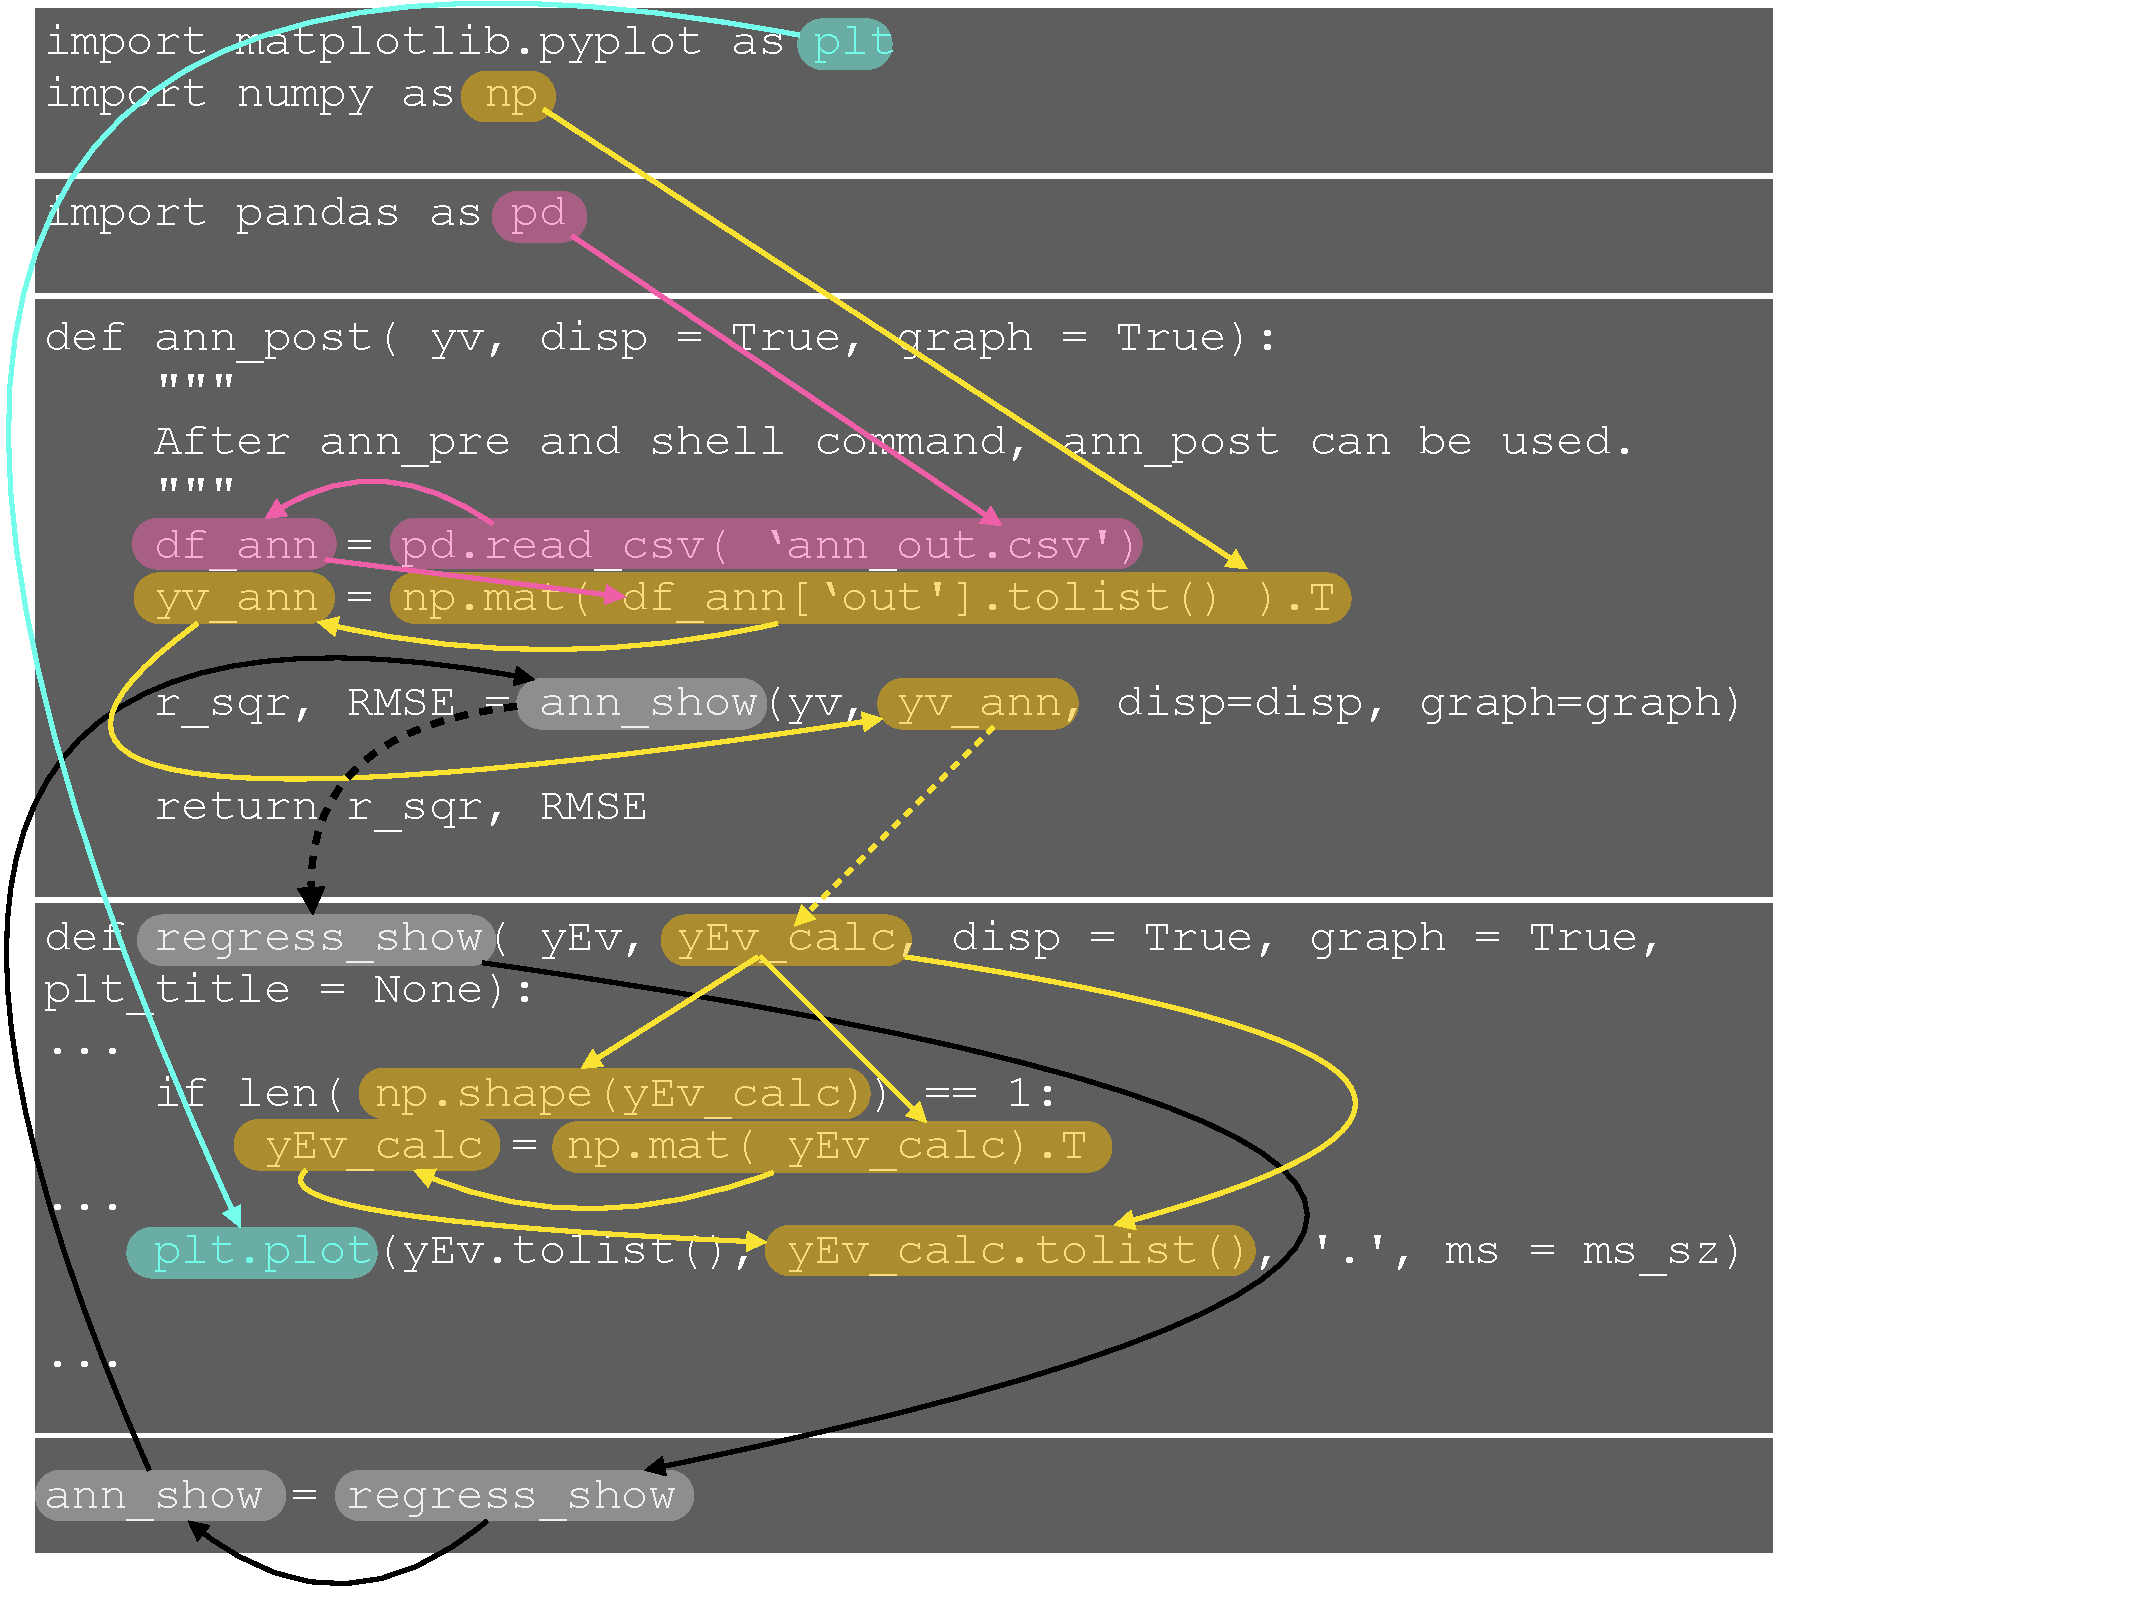
\includegraphics[width=5in]{paper_figures/example_flow}
\end{center}
\caption{Dataflow in example}
\label{fig:code_graph}
\end{figure*}

 The first thing to note is that the code in this snippet is in five
disparate pieces spread over roughly 200 lines of the source file.  Techniques
based on source text or local structures such as ASTs or CFGs will not
be able to capture dependencies over this range.  Global structures like a
call graph and dataflow analysis can.  Consider the call to {\tt ann\_show} on
line~\ref{line:ann_show}; it clearly calls the function {\tt
regress\_show} since that function is assigned to {\tt ann\_show}.
Knowing this requires following the dataflow from the definition of
{\tt regress\_show}, to its subsequent read, to the definition of {\tt
ann\_show}, to its read.  Thus dataflow must be tracked globally
across disparate portions of the code, as illustrated by the black
lines and boxes in Figure~\ref{fig:code_graph}.  And the call graph
must reflect that the function called depends on this dataflow, since
the call is to {\tt regress\_show} due to the dataflow, as illustrated
with the dashed arrow.  This is all complicated by the dynamic
nature of Python, illustrated here by the assignment of the function
{\tt regress\_show} to the variable {\tt ann\_show} on
line~\ref{line:ann_show}.  Note that {\tt ann\_show} called on
line~\ref{line:plotcall} is not even a function at all, but rather a variable
assigned from the actual function.  Of the analysis frameworks that
support interprocedural analysis including first class functions,
relatively few have been applied to Python.  We use WALA, which has, and supports many languages such as Javascript and Java.

This snippet also illustrates the fact that user code tends to rely
heavily on imported library code, which is the main focus of what we
represent in the knowledge graph.  There are seven lines of user code,
and these lines make use of three libraries ---{\tt Pandas}, {\tt
Numpy}, {\tt Matplotlib}---and four functions from them---{\tt
read\_csv}, {\tt mat}, {\tt to\_list}, {\tt plot}---with {\tt
to\_list} being used three times.  The interplay of dataflow between
the user code and its library calls is intricate and crucial to
understanding dataflow.  Consider what is required even to know that
{\tt pyplot} is used on an object from {\tt numpy}, which is in turn
computed from data read by {\tt pandas}.  The first steps are
straightforward dataflow from the {\tt import} calls to {\tt np.mat}
and {\tt pd.read\_csv}, shown by a yellow and pink arrow respectively.
The result of {\tt read\_csv} is assigned to {\tt df\_ann}, which is
used as an argument to {\tt np.mat}, shown by pink arrows.  The {\tt
mat} returns some object created by {\tt numpy} and then its {\tt T}
field is extracted and assigned to {\tt yv\_ann}.  So {\tt yv\_ann} is
created by {\tt numpy}, show by a yellow arrow to it.  That same value
is used in the {\tt ann\_show} call, with another yellow arrow
connecting it.  We saw above how the call target was determined, so a
dashed yellow arrow connects argument {\tt yv\_ann} to parameter {\tt
yEv\_calc}.  The dataflow in {\tt regress\_show} is similar, with
dataflow via {\tt yEv\_calc} and another value from {\tt numpy}
created by {\tt np.mat}.  The last step is the dataflow from the {\tt
pyplot} import to the {\tt plt.plot} call, where it is clear that a
call to {\tt pyplot} is using a value from {\tt numpy}.

The foregoing seems to assume we understand dataflow through the library
calls, but any actual model of code within the libraries will be daunting.  Any
actual analysis of the code must contend with a large code base in
multiple languages that are used to implement libraries.  
And any model will be difficult due to the sheer
scope of the libraries, with thousands of calls in each library alone.  There
is no formal static typing in this code to help; there is
idiosyncratic English API documentation of varying quality, but the
precise parametric semantics of functions like {\tt to\_list} is hard
to capture robustly in human- and machine-comprehensible English.  And
yet we need to capture enough library semantics to understand dataflow
at a high level.

To just approximate dataflow, we use an approach where 
the precise meanings of library calls do
not always matter as long as we track the flow of objects between
different calls.  For instance, since we want to capture that {\tt
plot} is used on the result of a {\tt mat} call, we need to track
data flow.  We really want an object that represents whatever it may
be that {\tt mat} returns.  Beyond that, we need to follow accesses to
that object, such as the read of {\tt T} on line~\ref{line:mat}.  To
do this, we introduce turtle objects: every library call returns a fresh
turtle, and accesses to properties---such as {\tt T}--- return the
same unknown object as its container.  Thus the calls on {\tt
  read\_csv}, {\tt mat}, {\tt to\_list}, and {\tt plot} all return new
turtle objects.  On the other hand, user code objects, such as the
function {\tt regress\_show} are treated normally.  As we show, this
mechanism allows us to track data flow with sufficient precision
without needing to model APIs at all.  Approximate analysis is what we use to scale analysis to many thousands of library calls in building our knowledge graph.


\subsection{validation of the knowledge graph}
Hold back 10\% edges of the graph, can we predict the other 90\%
\section{Mining Documentation associated with code}
This section will contain mining docstrings, associating it with turtles using inferencing?, mining RST/MD files, mining Stack overflow
\subsection{validation of the documentation?? how might we validate?}
\section{WhyIs} An introduction to what is our framework for the graph, and why we need such a framework.  What are the pieces of functionality on the graph that this enables. Visualization, demo, query access, provenance 
\section{statistics on the knowledge graph}
How many nodes and edges are in the graph, how many are connected to doc, how many are connected to usage etc


\bibliographystyle{ACM-Reference-Format}
\bibliography{sample-bibliography}

\end{document}
